\section{Module B — Clustering K-Means et interprétation MINT/DGI}
\label{sec:module_b_clusters}

\subsection{Familles de plaques identifiées}

\textbf{Portée et limite assumées} : la vision par ordinateur ne peut pas, à
elle seule, constater un statut administratif (vignette expirée, plaque
falsifiée) — ce sont des faits qui dépendent d'un registre DGI/MINT, pas
d'une propriété de l'image. Le clustering porte donc sur des features de
\textbf{qualité/lisibilité visuelle} mesurables objectivement : netteté
(variance du Laplacien), contraste, nombre de caractères segmentables et
confiance OCR (voir \texttt{modules/module\_b/plate\_quality\_features.py}).

L'algorithme K-Means appliqué à ces 4 features a produit $k=3$ clusters
sur un corpus de 4791 plaques (source Roboflow uniquement —
seule source disposant d'une annotation réelle de localisation de la plaque).
Chaque cluster est ordonné par qualité décroissante (cluster~0 = la plus
lisible) puis nommé selon les procédures opérationnelles MINT/DGI Cameroun
détaillées en §\ref{sec:procedures_mint_dgi}.

\begin{table}[H]
    \centering
    \caption{Clusters K-Means — interprétation MINT/DGI (Module B)}
    \label{tab:clusters_mint_dgi}
    \small
    \begin{tabular}{c|p{3cm}|r|r|r|r|p{2.4cm}|c|c}
        \hline
        \textbf{ID} & \textbf{Famille} & \textbf{N} & \textbf{\%} &
        \textbf{Dist.} & \textbf{Conf.H\%} & \textbf{Ex. plaques OCR} &
        \textbf{Autorité} & \textbf{Action MDP} \\
        \hline
        0 & Plaque nette / lisible & 810 & 16.9\% & 1.47 & 22.1\% & SHK462HB, GGE950FV, KSF897HG & — & \texttt{PASS} \\
        \hline
        1 & Plaque dégradée / lisibilité partielle & 2449 & 51.1\% & 1.43 & 24.2\% & PE13460, 8EEALLL, VA888J8A & MINT & \texttt{ALERT_MINT} \\
        \hline
        2 & Plaque illisible / fortement dégradée & 1532 & 32.0\% & 1.07 & 52.9\% & 2, SRZSZBJ, TRNOGHH & DGI & \texttt{ALERT_DGI} \\
        \hline
    \end{tabular}
\end{table}

\subsection{Validation de la séparation des clusters}

Il n'existe pas de vérité-terrain "plaque conforme/dégradée/illisible" dans
ce dataset (statut visuel, pas administratif). On valide donc uniquement que
les clusters \textbf{séparent bien le signal de qualité} mesuré, via un repère
binaire indépendant simple — "l'OCR a renvoyé un texte non vide" :
\begin{itemize}
    \item \textbf{ARI} (Adjusted Rand Index) : $0.0449$ —
    mesure la concordance entre partitions (0 = aléatoire, 1 = parfait).
    \item \textbf{NMI} (Normalized Mutual Information) : $0.1212$ —
    mesure l'information partagée entre les deux partitions.
\end{itemize}

Ces valeurs restent modestes et partiellement circulaires (la confiance OCR a
servi à construire le cluster) — elles ne prouvent pas une détection de
fraude, seulement que les paliers de qualité sont cohérents avec un signal
de lisibilité indépendant (voir figure~\ref{fig:cluster_vs_labels_interp},
qui montre la séparation des 4 features par cluster).

\begin{figure}[H]
    \centering
    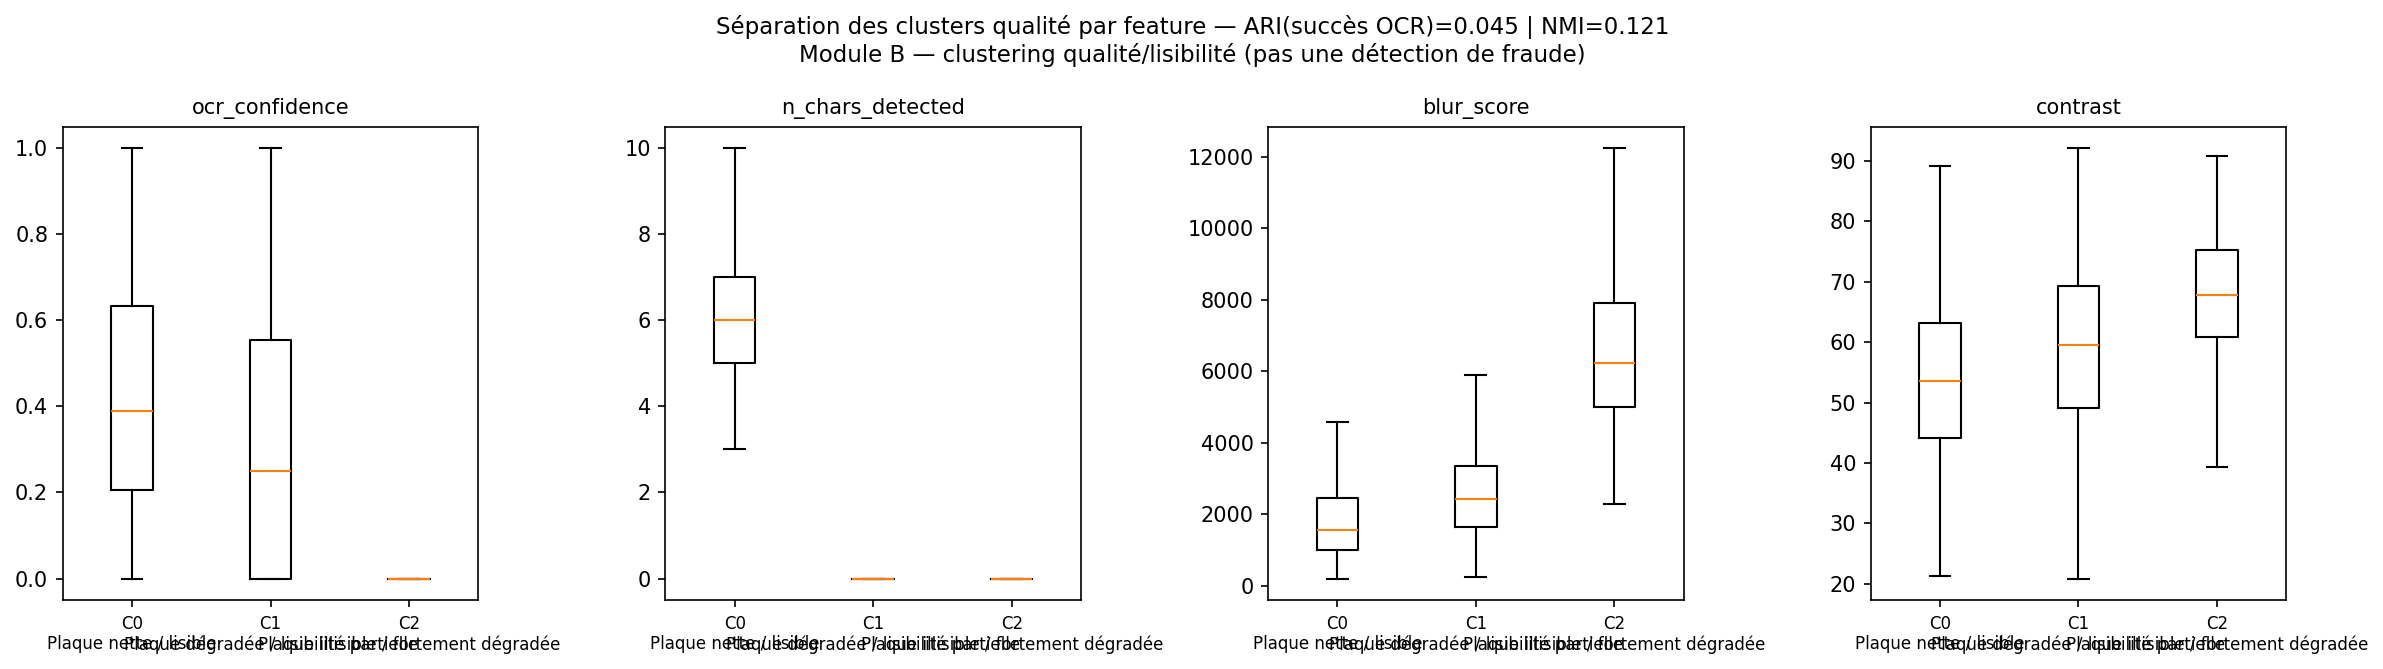
\includegraphics[width=0.85\textwidth]{figures/cluster_vs_labels_interp.png}
    \caption{Séparation des features de qualité par cluster K-Means —
    Module B (ARI=0.045, NMI=0.121 vs. succès OCR)}
    \label{fig:cluster_vs_labels_interp}
\end{figure}

\subsection{Niveaux de confiance et états MDP (§4.3)}

La distance au centroïde de chaque image est discrétisée en trois niveaux
par terciles globaux :
\begin{itemize}
    \item \textbf{Confiance haute} (niveau 0, $d \leq q_{33}$) :
    image proche du centroïde — assignation fiable.
    \item \textbf{Confiance moyenne} (niveau 1, $q_{33} < d \leq q_{66}$).
    \item \textbf{Confiance faible} (niveau 2, $d > q_{66}$) :
    cas ambigu — recours humain recommandé.
\end{itemize}

En combinant les $k=3$ clusters, les 3 niveaux de confiance
et le signal d'alerte binaire OCR, on obtient
$k \times 3 \times 2 = 18$ états MDP pour le Module C
(§\ref{sec:module_c_mdp}).

\begin{figure}[H]
    \centering
    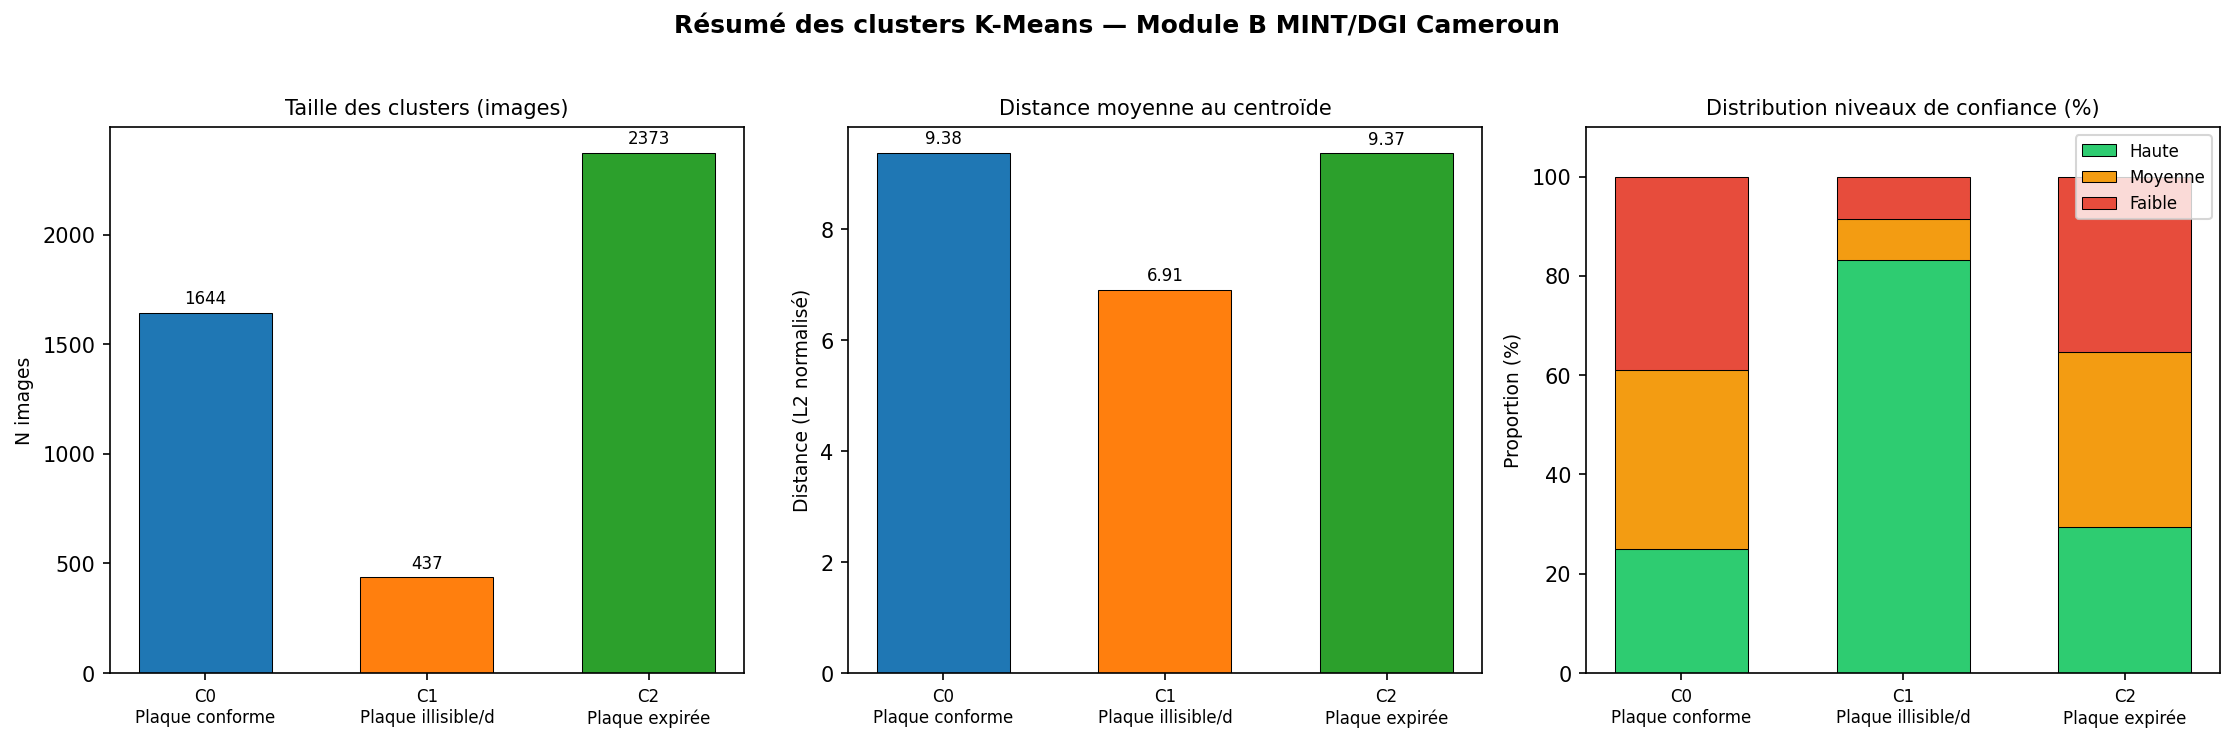
\includegraphics[width=0.85\textwidth]{figures/cluster_summary.png}
    \caption{Résumé des clusters K-Means — taille, confiance et procédure MINT/DGI}
    \label{fig:cluster_summary}
\end{figure}
